% intro

Basic concept in GeoPAT 2.0 is to divide a raster into a regular grid of motifels.
This grid encapsulate a complex content - a pattern corresponding to composition and spatial
configuration of cells in each motifels.
For the geoprocessing operations, such as search and comparison, a grid of motifels has a simple rectangular grid topology (left panel in Figure \ref{FIG:TOPO1}). 

\begin{figure}[H]
	\centering
	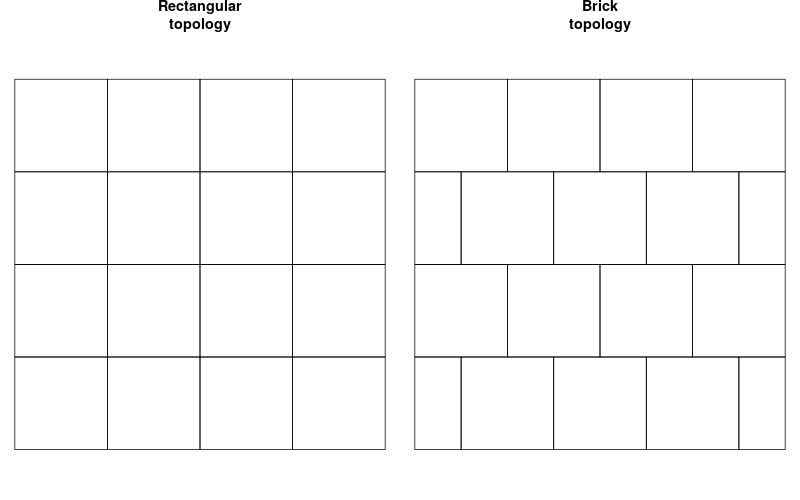
\includegraphics[width=\textwidth]{topology1.png}
	\caption{Two possible topologies for a grid of motifels: rectangular (4-connected grid) and brick (6-connected grid)}
	\label{FIG:TOPO1}
\end{figure}

This representation is simple and useful in many cases.
However, it also has significant shortcomings for task such as segmentation.
Due to its 4-connectivity, segmentation based on the rectangular topology often results in a large number of small (usually one-motifel size) segments.
% reference to the segmentation paper
To solve this issues, the 6-connected brick topology was created (right panel in Figure \ref{FIG:TOPO1}).
Square motifels are arranged in alternative layers, where each layer is shifted by a half of size of output motifel.
% reference to the segmentation paper

The {\tt gpat\_gridhis} module creates objects only in the rectangular (4-connected grid) topology. 
However, {\tt gpat\_segment} uses the brick (6-connected grid) topology during its segmentation procedure as a default.
(Note: it is possible to use the rectangular topology in the segmentation procedure by adding the {\it -q} flag).
It this process, neighboring motifels are merged to create the brick wall topology (Figure \ref{FIG:TOPO2}).
Importantly, this influence the size and shift of motifels and therefore change a size of analyzed area.

\begin{figure}[H]
	\centering
	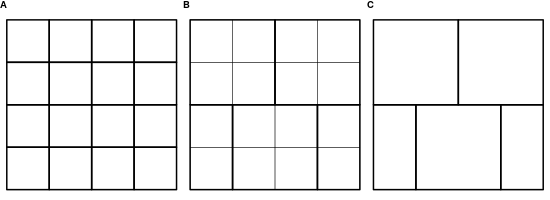
\includegraphics[width=\textwidth]{topology2.png}
	\caption{Process of merging elements of the rectangular topology to the brick topology: (A) input grid in the rectangular topology, (B) neighboring motifels in the rectangular topology are merged to create the brick wall topology, (C) output grid in the brick topology}
	\label{FIG:TOPO2}
\end{figure}

For example, we created a new grid using {\tt gpat\_gridhis} with the size and shift arguments set to 100.
This means that each motifel encapsulates pattern in an area of 9 sq km (one cell size is 30 meters; 30 meters x 100 = 3 km; 3 km * 3km = 9 sq km).
However, the segmentation module uses the brick topology as a default.
Thus, neighboring motifels are merged and create a new "brick" motifels.
This time each motifel encapsulates pattern in an area of 36 sq km (9 sq km motifels are combined into quadruples).
This means that if we want to segment patterns in scale of 9 sq km, we need to create a new grid of the size and shift twice smaller - 50.

\begin{figure}[H]
	\centering
	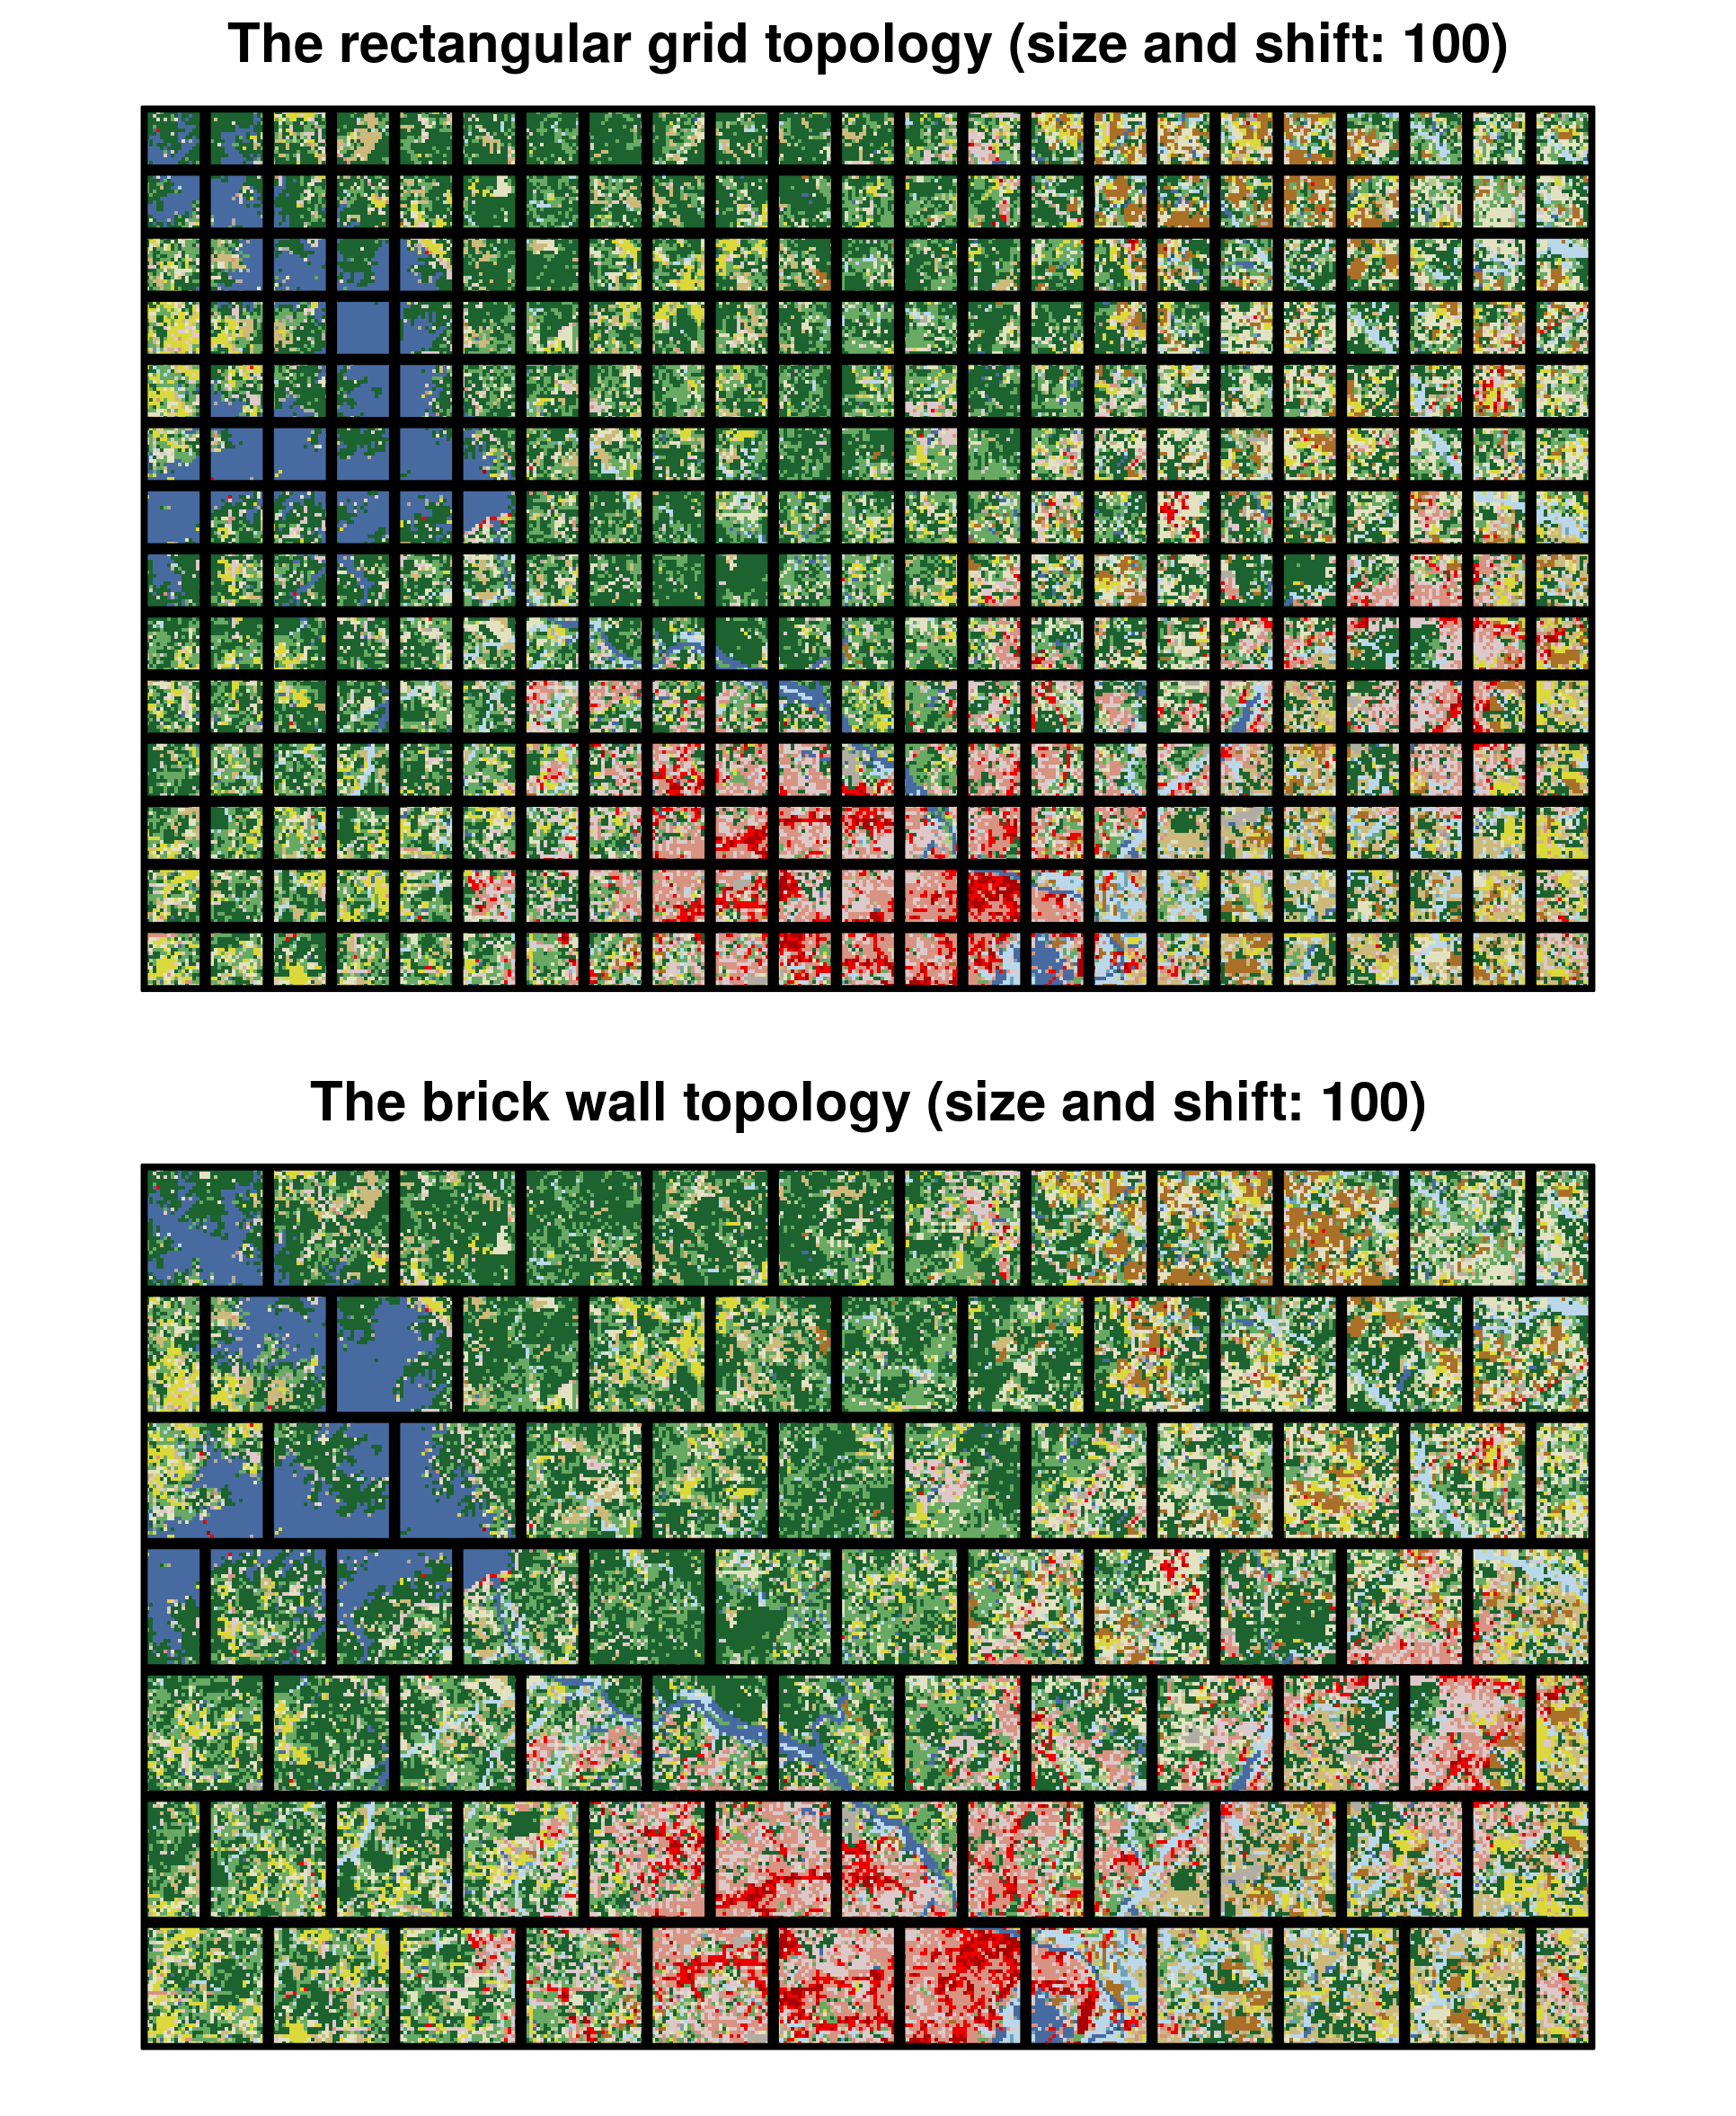
\includegraphics[width=\textwidth]{topology100.png}
	\caption{Comparision between the rectangular grid topology and the brick topology for Augusta}
	\label{FIG:TOPO3}
\end{figure}

